\definecolor{Purple}{RGB}{120,28,129}
\definecolor{Blue}{RGB}{63,96,174}
\definecolor{Duck}{RGB}{83,158,182}
\definecolor{Green}{RGB}{109,179,136}
\definecolor{Yellow}{RGB}{202,184,67}
\definecolor{Orange}{RGB}{231,133,50}
\definecolor{Red}{RGB}{217,33,32}
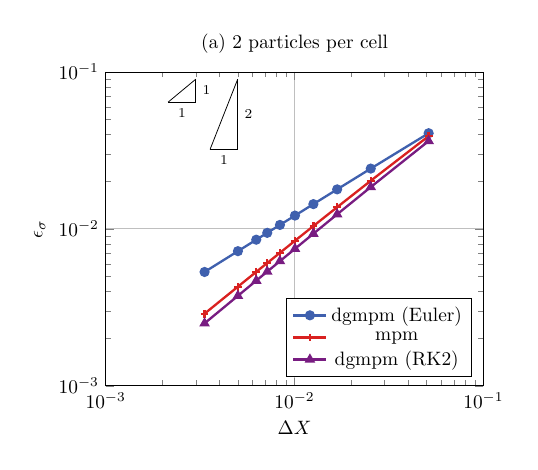
\begin{tikzpicture}[scale=0.7]
\begin{loglogaxis}[xlabel=$\Delta X$,ylabel=$\epsilon_\sigma$,ymajorgrids=true,xmajorgrids=true,legend pos=south east,title={(a) 2 particles per cell},xmin=0.001,xmax=0.1,ymin=0.001,ymax=0.1]
\addplot[Blue,very thick,mark=*] coordinates {(0.05128205128205128,0.04071623287797973) (0.025316455696202535,0.02422331391970186) (0.01680672268907563,0.017859682981968106) (0.012578616352201259,0.014382679392589382) (0.010050251256281405,0.01215794971476289) (0.008368200836820083,0.010597810573269258) (0.007168458781362007,0.0094358643935967) (0.006269592476489028,0.008532797475738967) (0.005012531328320802,0.007212428097178037) (0.00333889816360601,0.005314181157028796) };
\addplot[Red,very thick,mark=+] coordinates {(0.05128205128205128,0.0390291535717384) (0.025316455696202535,0.020268530894136598) (0.01680672268907563,0.013750393207018721) (0.012578616352201259,0.010423623198621649) (0.010050251256281405,0.008401372949263077) (0.008368200836820083,0.007040635899883742) (0.007168458781362007,0.006061777084922055) (0.006269592476489028,0.005323473586831238) (0.005012531328320802,0.004283201972277798) (0.00333889816360601,0.0028821343862208276) };
\addplot[Purple,very thick,mark=triangle*] coordinates {(0.05128205128205128,0.03630880169702076) (0.025316455696202535,0.018472488539206525) (0.01680672268907563,0.012386226022652155) (0.012578616352201259,0.009316464511847778) (0.010050251256281405,0.007466054839937482) (0.008368200836820083,0.006228877333241853) (0.007168458781362007,0.005343427654516536) (0.006269592476489028,0.00467838164898954) (0.005012531328320802,0.003745935463601613) (0.00333889816360601,0.0025001637383401188) };
\legend{dgmpm (Euler),mpm,dgmpm (RK2)}
\draw (axis cs:0.003,0.09) -- (axis cs:0.003/1.4,0.09/1.4);
\draw (axis cs:0.003,0.09) -- (axis cs:0.003,0.09/1.4) node [midway,right] {\scriptsize 1};
\draw (axis cs:0.003,0.09/1.4) -- (axis cs:0.003/1.4,0.09/1.4) node [midway,below] {\scriptsize 1};
\draw (axis cs:0.005,0.09) -- (axis cs:0.005/1.4,0.09/2.8);
\draw (axis cs:0.005,0.09) -- (axis cs:0.005,0.09/2.8) node [midway,right] {\scriptsize 2};
\draw (axis cs:0.005,0.09/2.8) -- (axis cs:0.005/1.4,0.09/2.8) node [midway,below] {\scriptsize 1};
\end{loglogaxis}
\end{tikzpicture}
